\documentclass{beamer}

\mode<presentation>
{
  \usetheme{default}
  \usecolortheme{dove}
  \usefonttheme{default}
  \setbeamertemplate{navigation symbols}{}
  \setbeamertemplate{caption}[numbered]
} 

\usepackage[english]{babel}
\usepackage[utf8x]{inputenc}
\usepackage{listings}

\definecolor{graybg}{RGB}{42,42,42}
\definecolor{titlecolor}{RGB}{115,185,0}
\definecolor{textcolor}{RGB}{232,232,232}

\setbeamercolor{background canvas}{bg=graybg}
\setbeamercolor{titlelike}{fg=titlecolor}
\setbeamercolor{frametitle}{fg=titlecolor}
\setbeamercolor{normal text}{fg=textcolor}
\setbeamerfont{frametitle}{size=\Huge}
\setbeamerfont{framesubtitle}{size=\Large}
\setbeamertemplate{caption}{\raggedright\insertcaption\par}

\AtBeginSection[]{
	\begin{frame}
		\vfill
		\centering
		\begin{beamercolorbox}[center]{title}
			\Huge{\usebeamerfont{title}}\insertsectionhead
		\end{beamercolorbox}
		\vfill
	\end{frame}
}

\title{GPGPU programming\\General-purpose Processing on Graphics Processing Units}
\author{Robin Faury\\robinfaurypro@gmail.com}
\date{01-09-2023}

\begin{document}

\begin{frame}
\titlepage
\end{frame}

\begin{frame}{Introduction}
	\begin{itemize}
		\item The purpose of parallel processing
		\item What is a graphic card?
		\item Languages
		\item GPGPU usage in the industry
		\item Examples
		\item Q\&A
	\end{itemize}
\end{frame}

\section{The purpose of parallel processing}
\begin{frame}{Moore's Law}
	Every two years, the density of transistors in an integrated circuit doubles. That means we can compute the critical path of an algorithm faster.
	\begin{figure}
		
\includegraphics[scale=0.2]{figures/buzz1.jpg}
		\caption{\textit{To infinity and beyond!}}
	\end{figure}
	However, it's now to difficult to add smaller transistor so we prefer double processor. This will result in a redesign of our algorithms.
\end{frame}

\begin{frame}{Critical path}
	Sometimes, algorithms process data one by one. When applicable, it is necessary to find the critical path and execute it in parallel. Modern CPUs offer the ability to run some threads at the same time. However, CPUs don't have a lot of cores available. For massive parallel computation we will use GPUs.
	\begin{figure}
		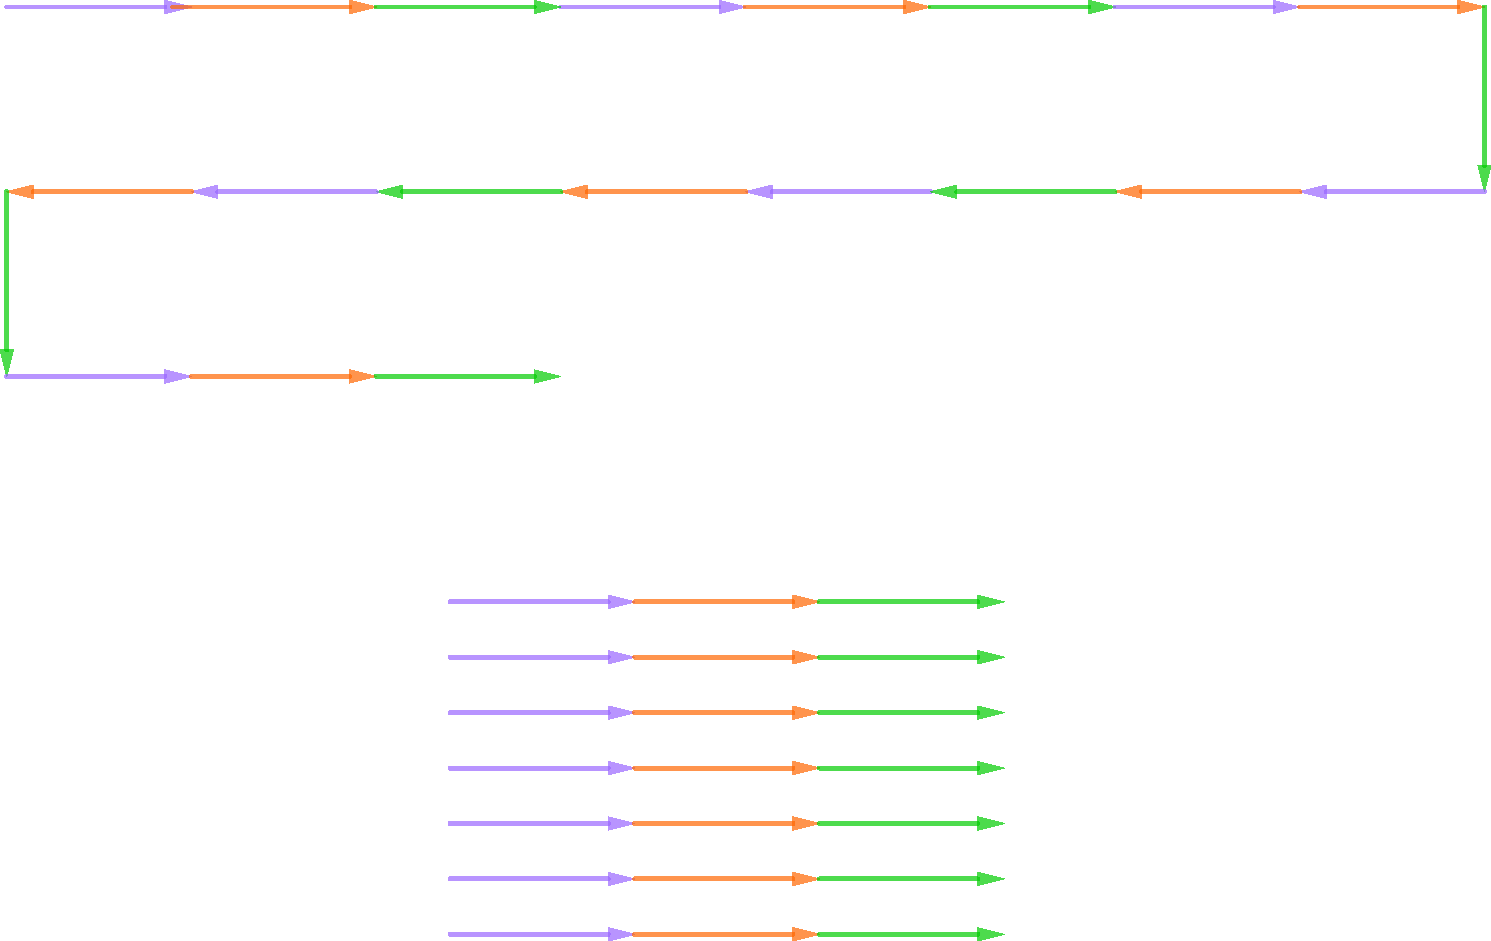
\includegraphics[scale=0.2]{figures/criticalPath.pdf}
	\end{figure}
\end{frame}

\begin{frame}{Latency and Throughput}
	\begin{itemize}
		\item \textbf{Latency:} This is the time between an action and the response to this action. For example, a key press event and its process.
		\item \textbf{Throughput:} This is the rate of production. For example, the number of pixels processed in one second.
	\end{itemize}
\end{frame}

\begin{frame}{CPU versus GPU}
	\begin{itemize}
		\item The aim of \textbf{CPU} is to be very responsive. For that they adopt strategies to hide the latency (pre-fetch, branch prediction...). However, these algorithms need a lot of memory cache.
		\item The aim of \textbf{GPU} is to process a lot of data. That why there is way more cores into GPU than CPU. The memory cache need to be divided by the number of cores.
	\end{itemize}
	A CPU has a small amount of thread, so it can dedicate a large cache to store intermediate result to be very responsive. A CPU has a low latency but a low throughput too.\\
	A GPU need a setup before running a process and he cannot store a lot of intermediate results but it can run a very large amount of thread. A GPU has a high latency but a high throughput too.
\end{frame}

\begin{frame}{Flynn's taxonomy}
	We just see two architectures to process data (the CPU and the GPU) but we can imagine other ones. Flynn made a classification of computer architectures.
	\begin{itemize}
		\item \textbf{SISD}: Single Instruction Single Data. One core of a CPU.
		\item \textbf{SIMD}: Single Instruction Multiple Data. A GPU.
		\item \textbf{MISD}: Multiple Instruction Single Data. An architecture that need to compute redundancy on a system.
		\item \textbf{MIMD}: Multiple Instruction Multiple Data. A distributed system.
	\end{itemize}
\end{frame}

\begin{frame}{SIMD: a world of buffers}
	General Purpose computing on GPU leverage the power of GPU to process a stream of data. All data will be store into a buffer and the solving of the arithmetic computation will be done from this buffer to another one (we can read/write a buffer but only in some specific cases). One process is called a kernel for the GPGPU or a shader for the graphics pipeline.
	\begin{figure}
		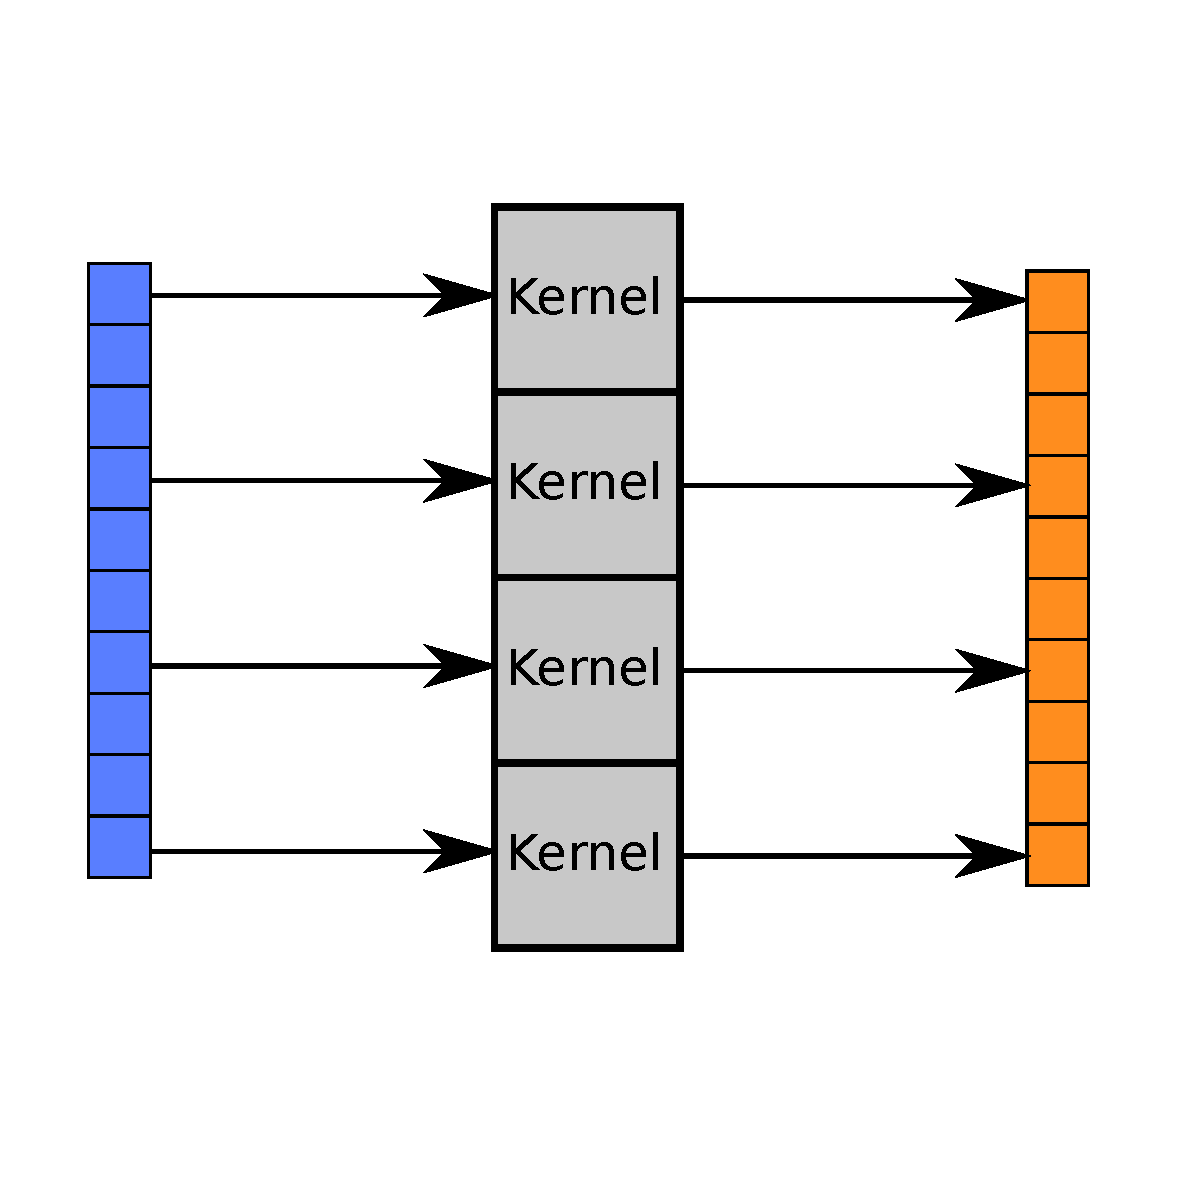
\includegraphics[scale=0.3]{figures/buffer.pdf}
	\end{figure}
\end{frame}

\begin{frame}{Host and Devices}
	\begin{itemize}
		\item Host: The CPU and its memory. The host can manage the memory on both the host and the device. The executed code can launch kernels.
		\item Devices: The GPU and its memory. Kernels are executed on many GPU threads in parallel.
	\end{itemize}
\end{frame}

\begin{frame}{Host and Device}
	A GPGPU need to be seen as an asynchronous service. The host (CPU) will send to a device (GPU) the assembly code of the process and then the data to process. The device don't need anymore information to work and the host is free to run other task. You have one host and one or more devices.
	\begin{figure}
		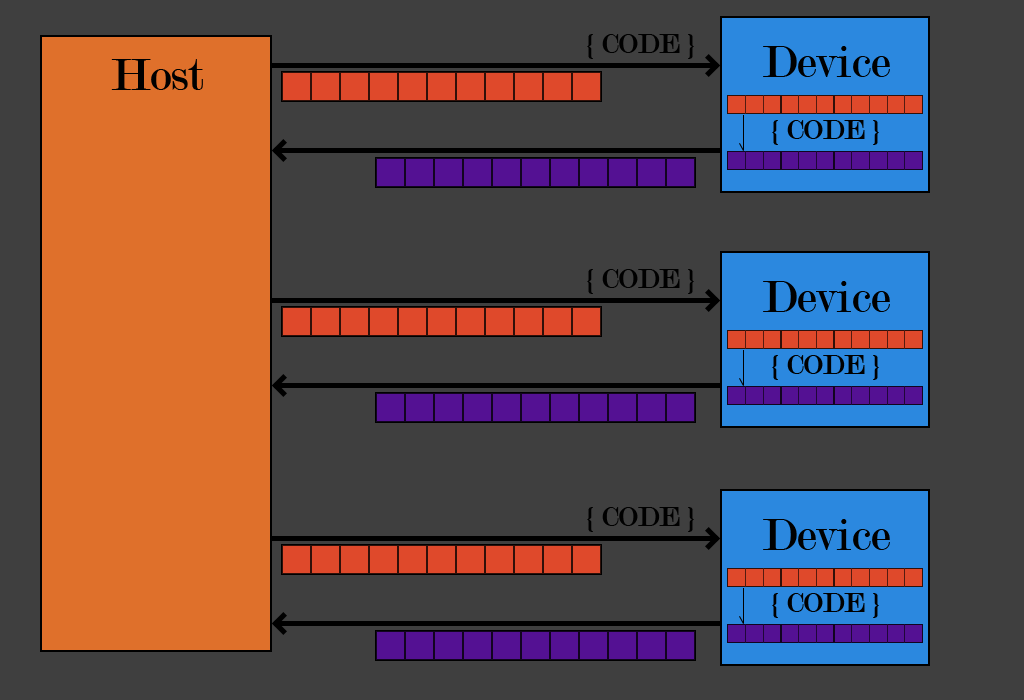
\includegraphics[scale=0.2]{figures/host_devices.png}
	\end{figure}
\end{frame}

\section{What is a graphic card?}
\begin{frame}{History}
	The first Graphics Processing Unit (GPU) was used for drawing game sprites. It was a dedicated device for formatted data. Ten years after we had the ability to draw lines, fill areas and control the blitter. In 1990, the graphical API appears and allows us to send assembly code to the device.
\end{frame}

\begin{frame}{Arithmetic Logic Unit}
	The Arithmetic Logic Unit (ALU) is the component that performs arithmetic operations. The GPU is more focused on floating point operations, multiple ALUs are combined to create a Floating Point Unit (FPU). Latest GPU include also dedicated chip for double operations.
	\begin{figure}
		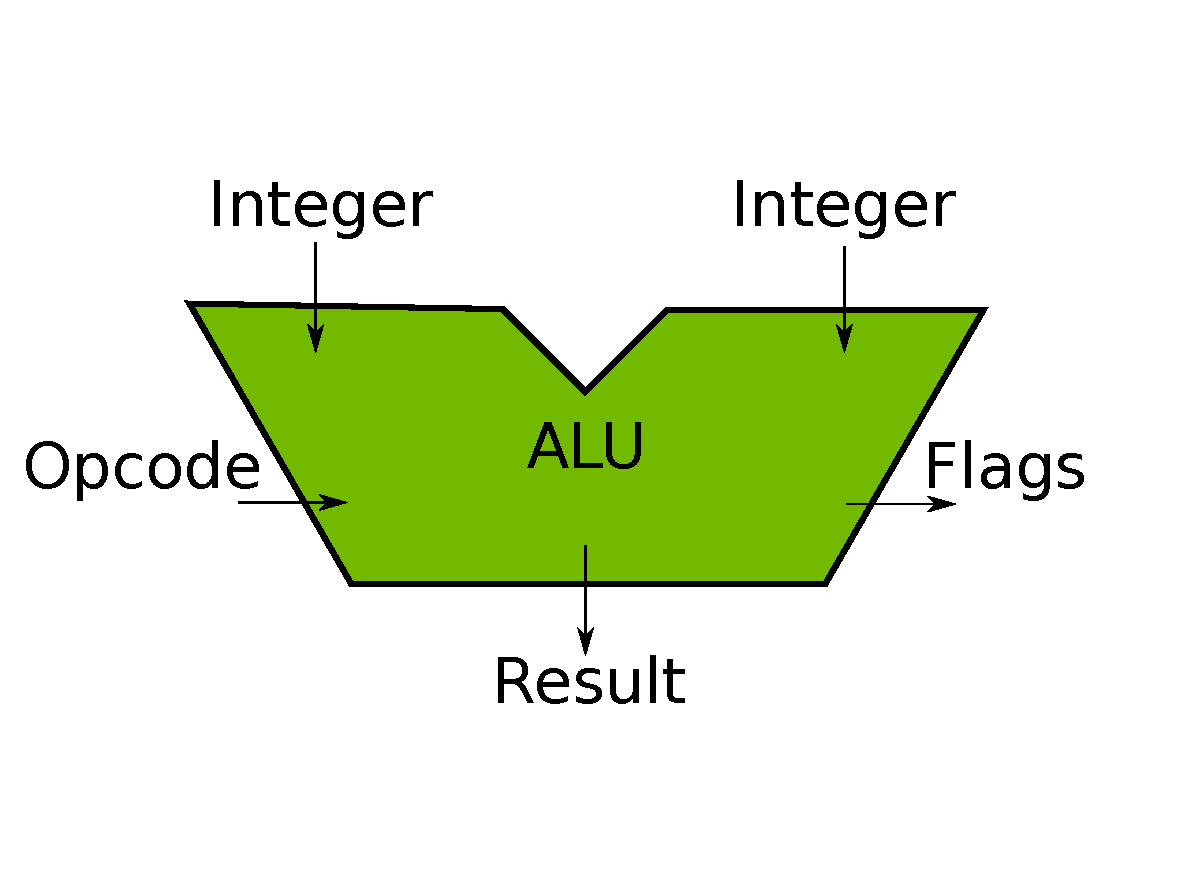
\includegraphics[scale=0.3]{figures/ALU.pdf}
	\end{figure}
\end{frame}

\begin{frame}{Core}
	Cores are used to execute opcodes from compiled kernels. There are composed of an FPU, logic unit, branch unit and compare unit.
	\begin{figure}
		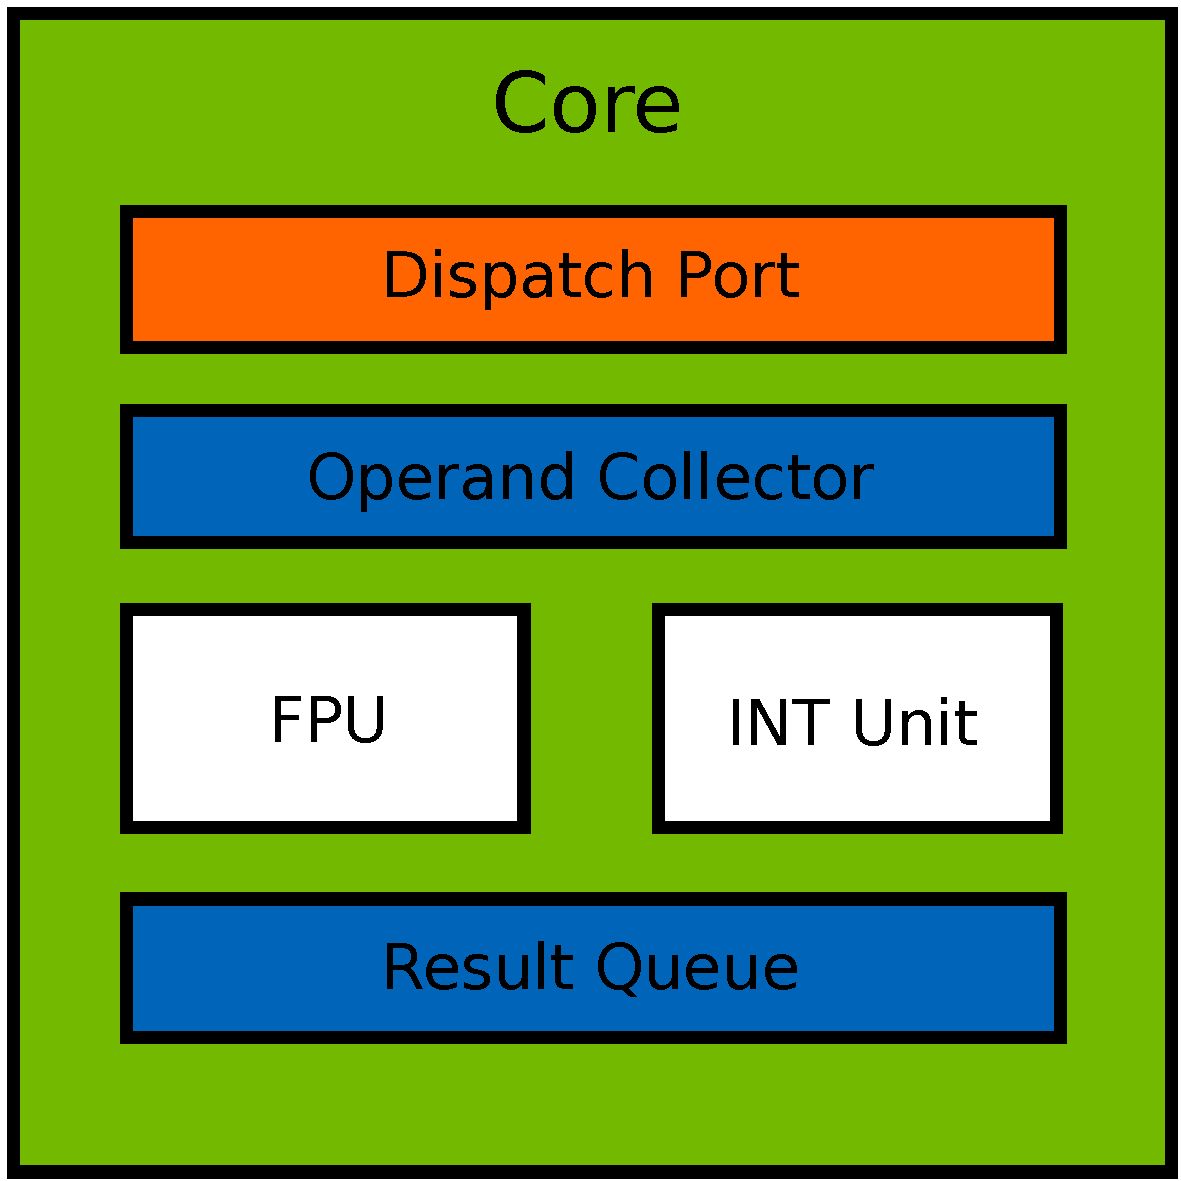
\includegraphics[scale=0.2]{figures/cudacore.pdf}
	\end{figure}
\end{frame}

\begin{frame}{Streaming Multiprocessor}
	The Streaming Multiprocessor (SM) organizes threads in groups of 32 called warp.
	\begin{figure}
		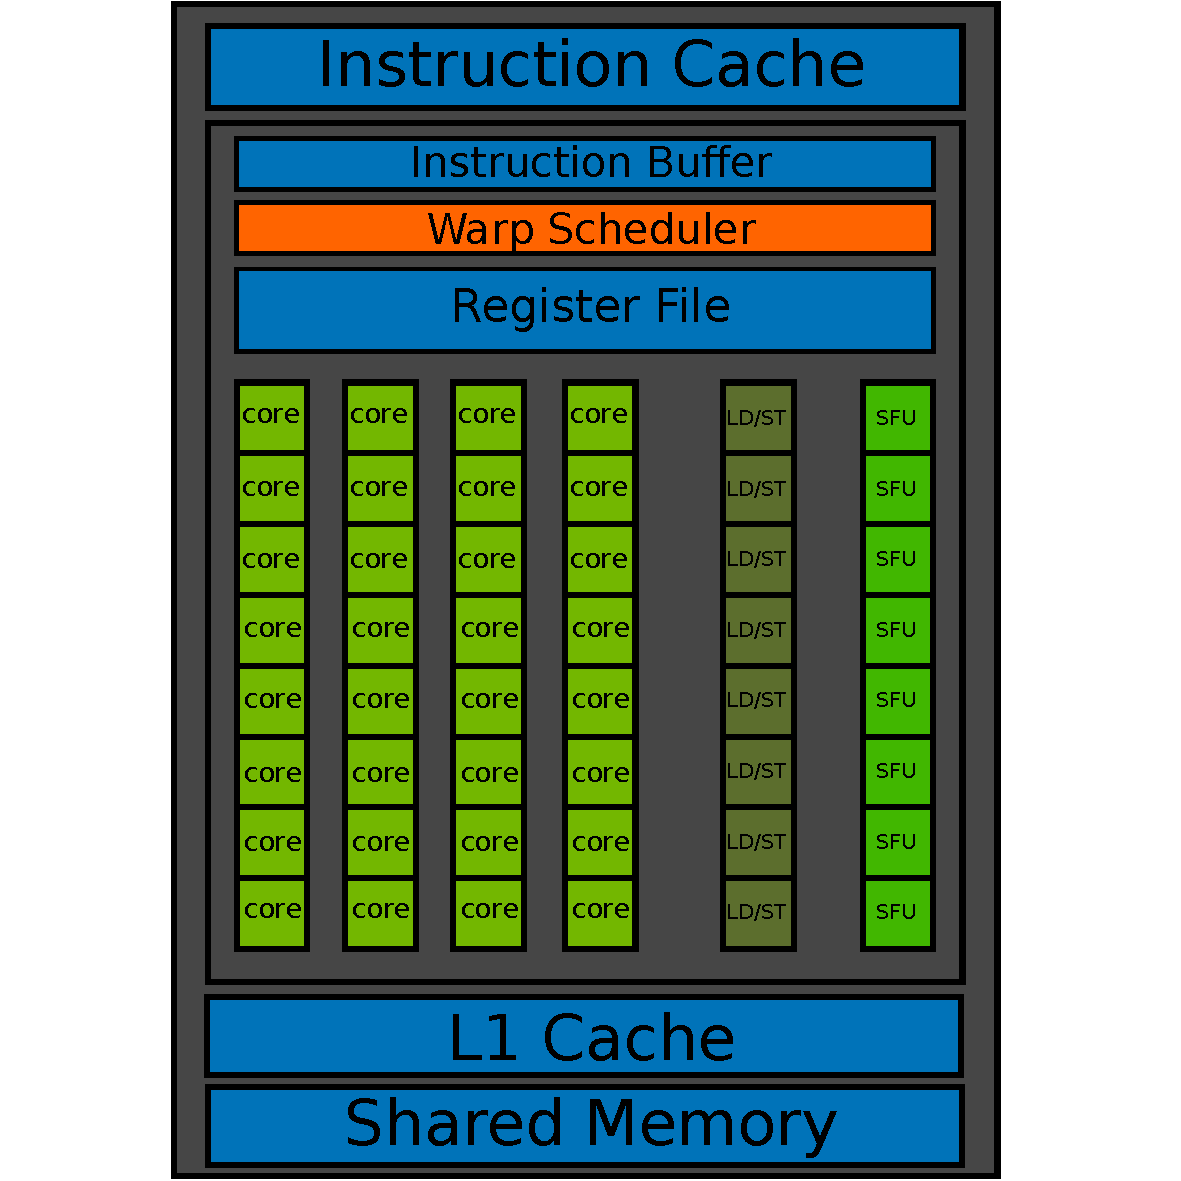
\includegraphics[scale=0.3]{figures/warp.pdf}
	\end{figure}
\end{frame}

\begin{frame}{Streaming Multiprocessor}
	On the GP104 (The GPU of GTX 1080) each SM has four warps. 
	\begin{figure}
		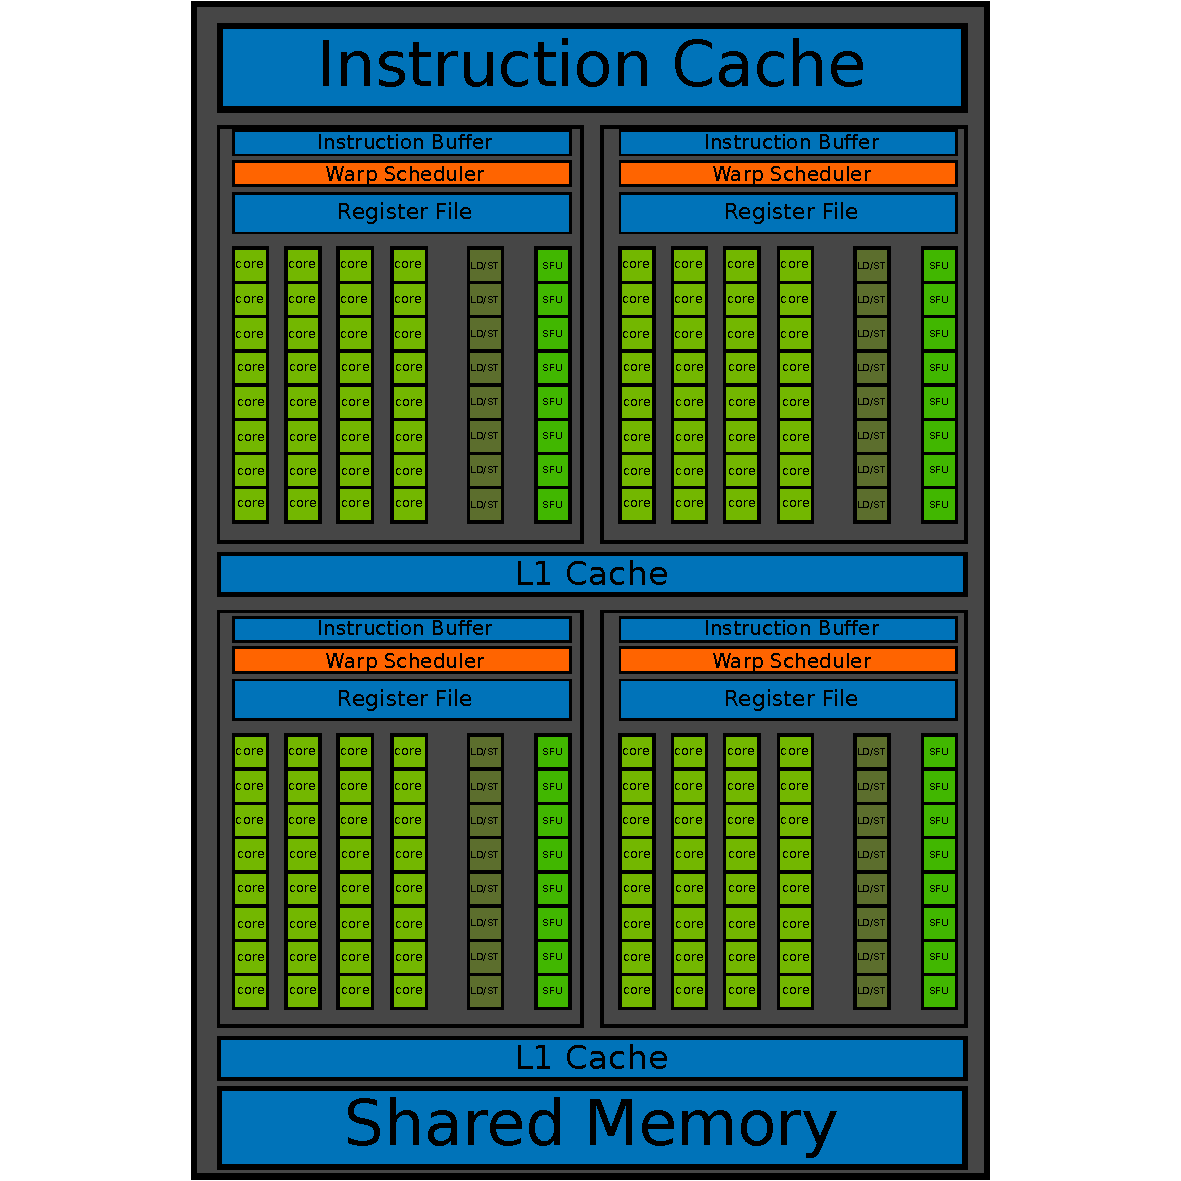
\includegraphics[scale=0.3]{figures/SM.pdf}
	\end{figure}
\end{frame}

\begin{frame}{Graphics Processing Clusters}
	A Graphics Processing Clusters (GPC) is a collection of streaming multiprocessors. In the case of the GP104, there are four clusters.
	\begin{figure}
		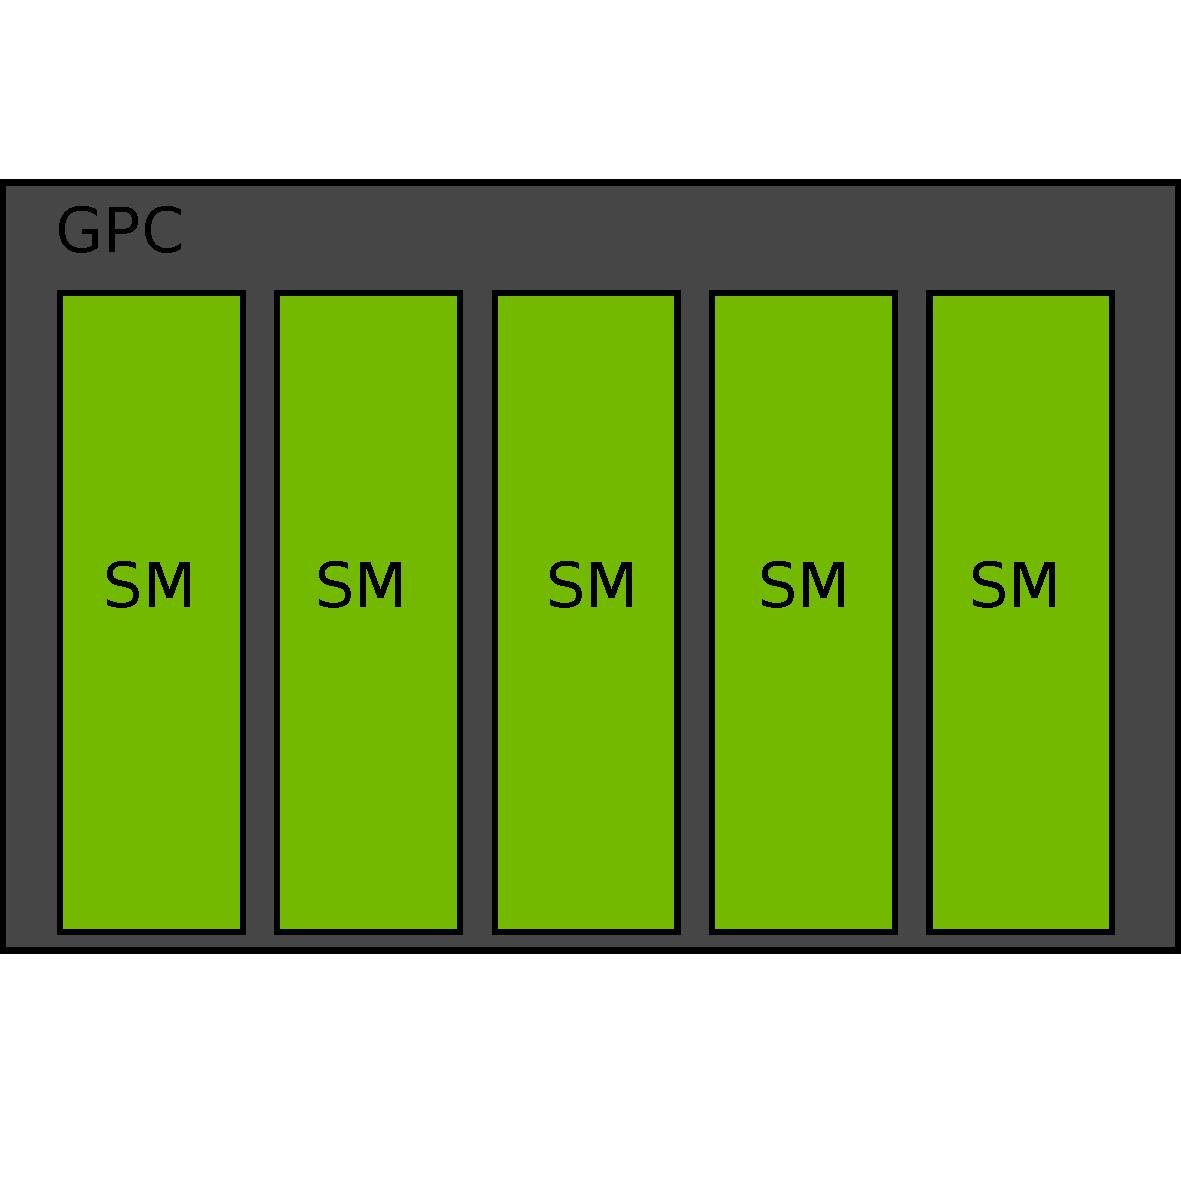
\includegraphics[scale=0.3]{figures/GPC.pdf}
	\end{figure}
\end{frame}

\begin{frame}{GP104}
	All the GPC are connected to the L2 cache memory. The Gigathread engine distributes block threads to streaming multiprocessor. This device has 32 cores * 4 warps * 5 SMs * 4 GPCs = 2560 CUDA cores.
	\begin{figure}
		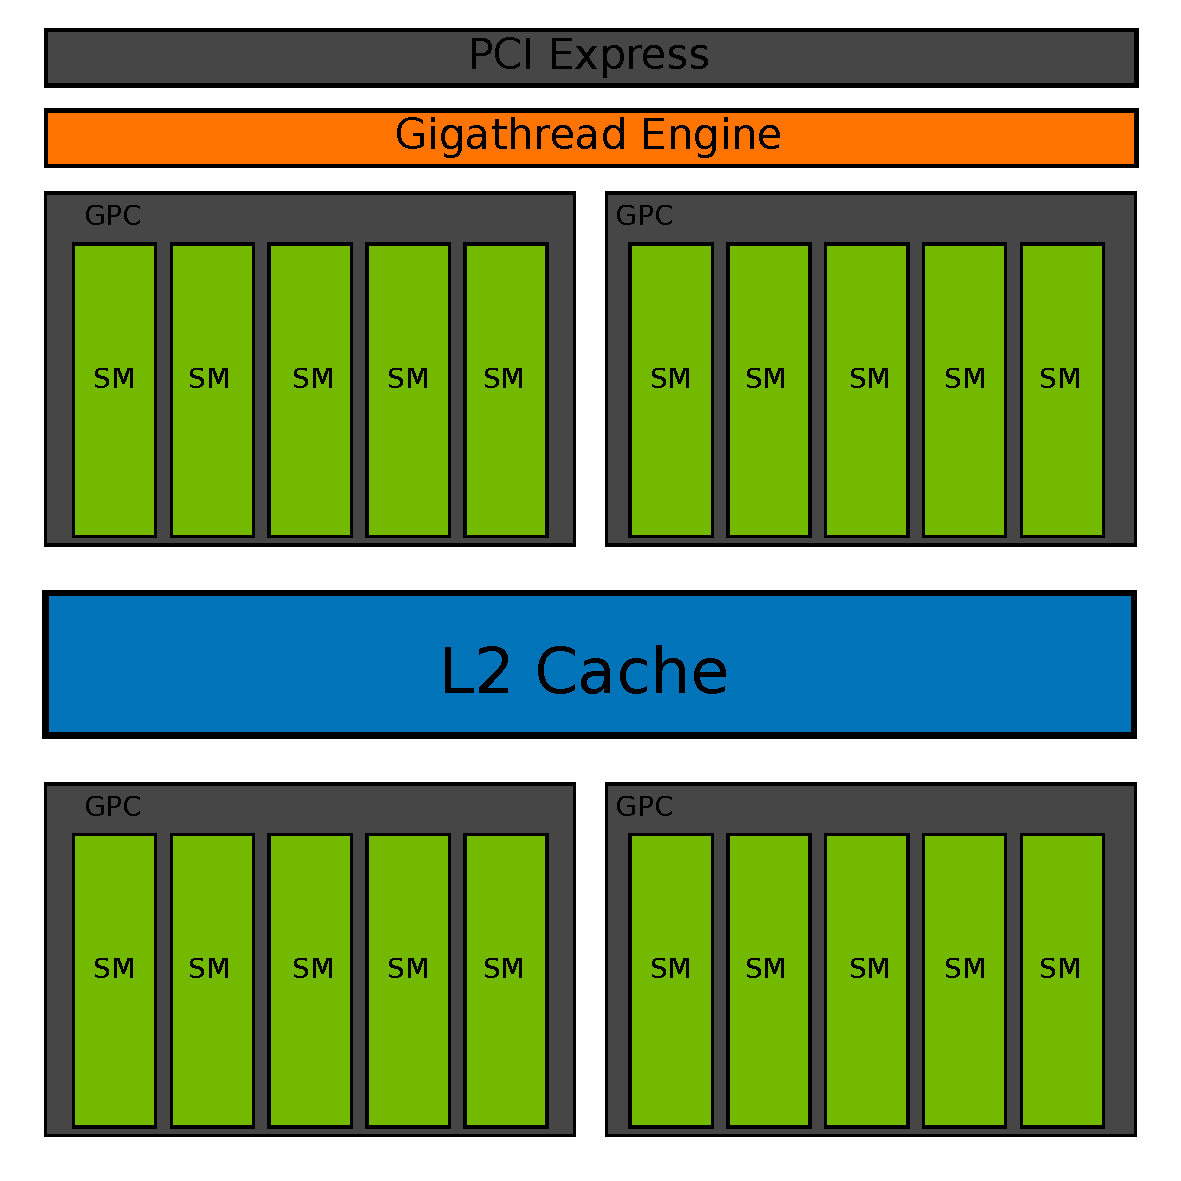
\includegraphics[scale=0.3]{figures/gp104.pdf}
	\end{figure}
\end{frame}

\begin{frame}{GA102}
	\begin{figure}
		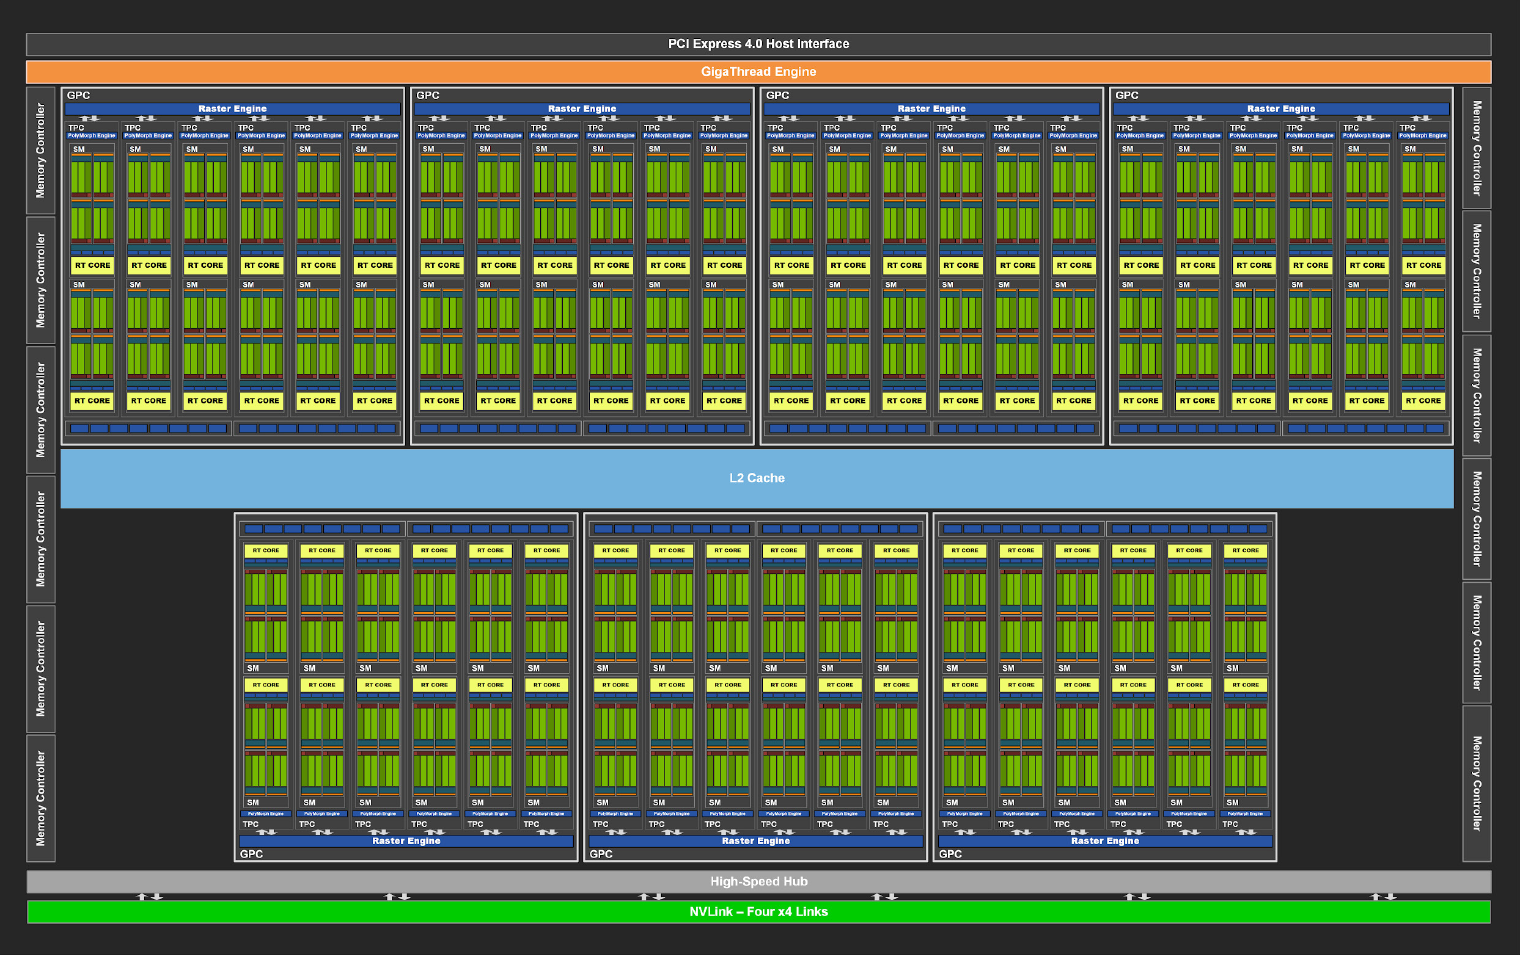
\includegraphics[scale=0.25]{figures/GA102.png}
	\end{figure}
\end{frame}

\section{GPGPU languages}
\begin{frame}{APIs}
	To communicate with the graphic card we need API. Each one have its pro and con.
	\begin{itemize}
		\item \textbf{CUDA:} The Nvidia API. Very close to the C++, easy to use. Works only on Nvidia card.
		\item \textbf{DirectX:} The Window API. Design for game development on Window.
		\item \textbf{Metal:} The Apple API. Design for graphic development on MacOS.
		\item \textbf{OpenGL:} Developed by Kronos, design for all OS. Deprecated from 2019.
		\item \textbf{Vulkan:} Developed by Kronos, design for all OS but MacOS. Launched on 2018. Difficult to use.
	\end{itemize}
\end{frame}

\begin{frame}{threads}
	A thread is the smallest sequence of programmed instructions that can be managed independently by a scheduler.
\end{frame}

\begin{frame}{Dispatch threads on CPU}
	On CPU, a task is a small independent function. It's also sometime call a job. Create a CPU thread is a very heavy process so most of the time, we create at the beginning of a program a unique thread pool. In a second time, we will send to the thread pool vectors of tasks. 8 (if the thread pool has 8 threads) tasks will be executed in parallel and others will be executed sequentially.
\end{frame}

\begin{frame}{Dispatch threads on GPU}
	From the host, you can dispatch a large amount of threads. In the same way threads are organized in lists in CPU, GPU threads are organized on a 3D grid. A kernel is a local 3D grid and a group is a global 3D grid. On a kernel we specify the number of invocation and when we use the dispatch function we specify the number of working group. Each working group will run x instance of the kernel.\\
	If we specify 42 invocations in the kernel code and we dispatch 1000 working groups, the GPU will run 42 000 threads.
\end{frame}

\lstset{language=C++,basicstyle=\ttfamily,keywordstyle=\color{red},commentstyle=\color{green},tabsize=1}

\defverbatim[colored]\codeKernelMain{
\begin{lstlisting}
	#version 430 core

	void main() {

	}
\end{lstlisting}
}

\begin{frame}{Kernel - GLSL}
	The kernel is the code that GPU will execute on the data. First it need the version of the GLSL language. It also need a main function.
	\codeKernelMain
\end{frame}

\defverbatim[colored]\codeKernelInvoc{
\begin{lstlisting}
	#version 430 core

	layout(
		local_size_x = 42,
		local_size_y = 1,
		local_size_z = 1) in;

	void main() {

	}
\end{lstlisting}
}

\begin{frame}{Kernel - GLSL}
	We can specify the number of invocation of the kernel. As you can see, the invocation can be set in 1D, 2D or 3D. It's useful if you work on buffer, texture or volume.
	\codeKernelInvoc
\end{frame}

\defverbatim[colored]\codeKernelBuffer{
\begin{lstlisting}
	#version 430 core

	layout(
		local_size_x = 42,
		local_size_y = 1,
		local_size_z = 1) in;

	layout(std140, binding = 0) buffer MyBuffer {
		float buffer_[];
	};

	void main() {

	}
\end{lstlisting}
}

\begin{frame}{Kernel - GLSL}
	If you need a input or an output buffer, you need to specify the following layout:
	\codeKernelBuffer
\end{frame}

\defverbatim[colored]\codeKernelBufferWrite{
\begin{lstlisting}
	#version 430 core

	layout(
		local_size_x = 42,
		local_size_y = 1,
		local_size_z = 1) in;

	layout(std140, binding = 0) buffer MyBuffer {
		float buffer_[];
	};

	void main() {
		float data=buffer_[gl_GlobalInvocationID.x];
		++data;
		buffer_[gl_GlobalInvocationID.x]=data;
	}
\end{lstlisting}
}

\begin{frame}{Kernel - GLSL}
	And finally, we can read/write this buffer.
	\codeKernelBufferWrite
\end{frame}

\defverbatim[colored]\codeIndex{
\begin{lstlisting}
	int index = blockIdx * blockDim + threadIdx;
\end{lstlisting}
}

\defverbatim[colored]\codeIndexDim{
\begin{lstlisting}
	int x = blockId.x * blockDim.x + threadId.x;
	int y = blockId.y * blockDim.y + threadId.y;
	int z = blockId.z * blockDim.z + threadId.z;
\end{lstlisting}
}

\begin{frame}{Indexing}
	In the last example, we use the GlobalInvocationID variable as the index of our buffer. This value can be computed using the WorkGroupID * WorkGroupSize + LocalInvocationID;
\end{frame}

\begin{frame}{Indexing with CUDA}
	GPGPU API are very similar. This is the way to have the thread index in CUDA:
	In the kernel, the thread Id, the block Id and the blockDim allow the user to compute the unique thread id.
	\codeIndex
	If data is stored into 2D or 3D array, it is possible to launch the kernel using a 3d vector instead of an integer and the index becomes:
	\codeIndexDim
\end{frame}

\begin{frame}{Indexing overview}
	\begin{figure}
		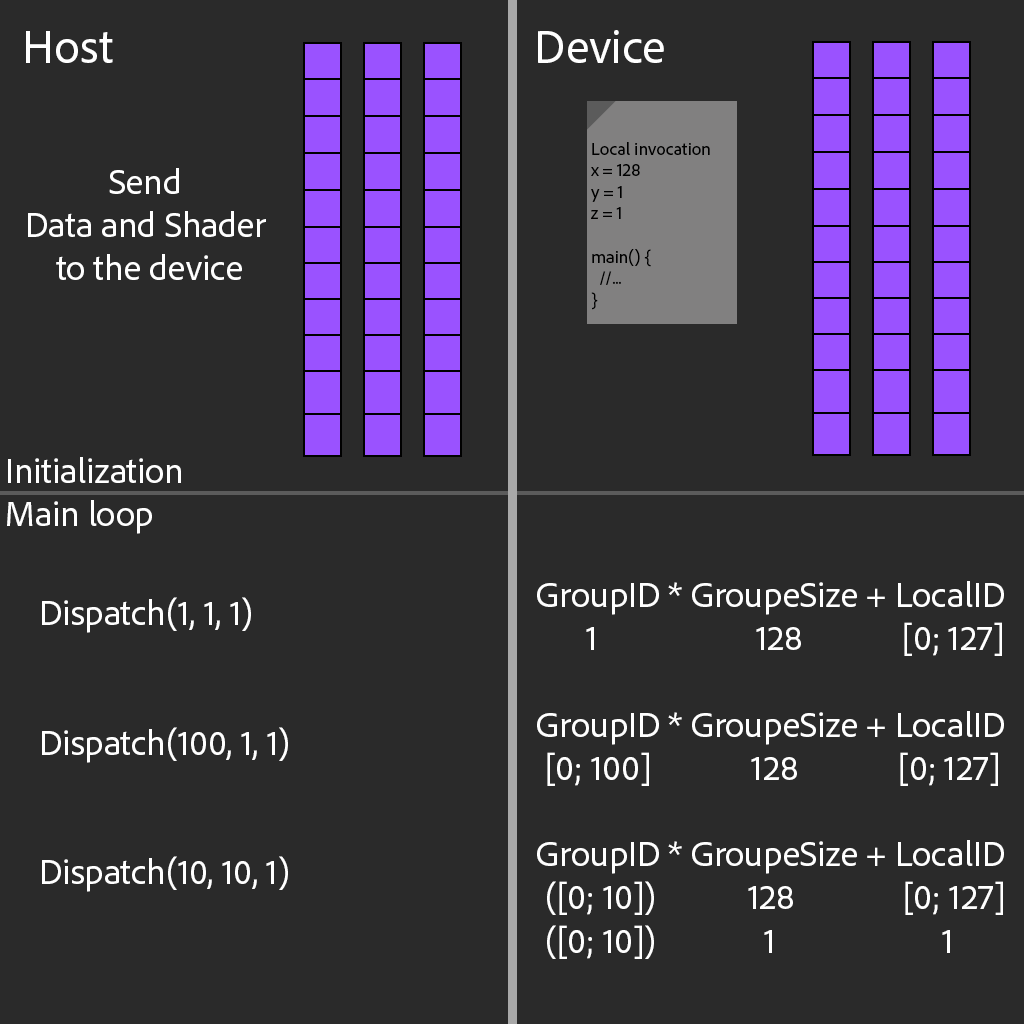
\includegraphics[scale=0.2]{figures/threadID.png}
		\caption{Relation between the CPU dispatch function and the ThreadID}
	\end{figure}
\end{frame}

\section{GPGPU usage in the industry}
\begin{frame}{APOD}
	The Assess, Parallelize, Optimize, Deploy (APOD) design cycle's goal is to identify and correct bottlenecks into the application. 
	\begin{figure}
		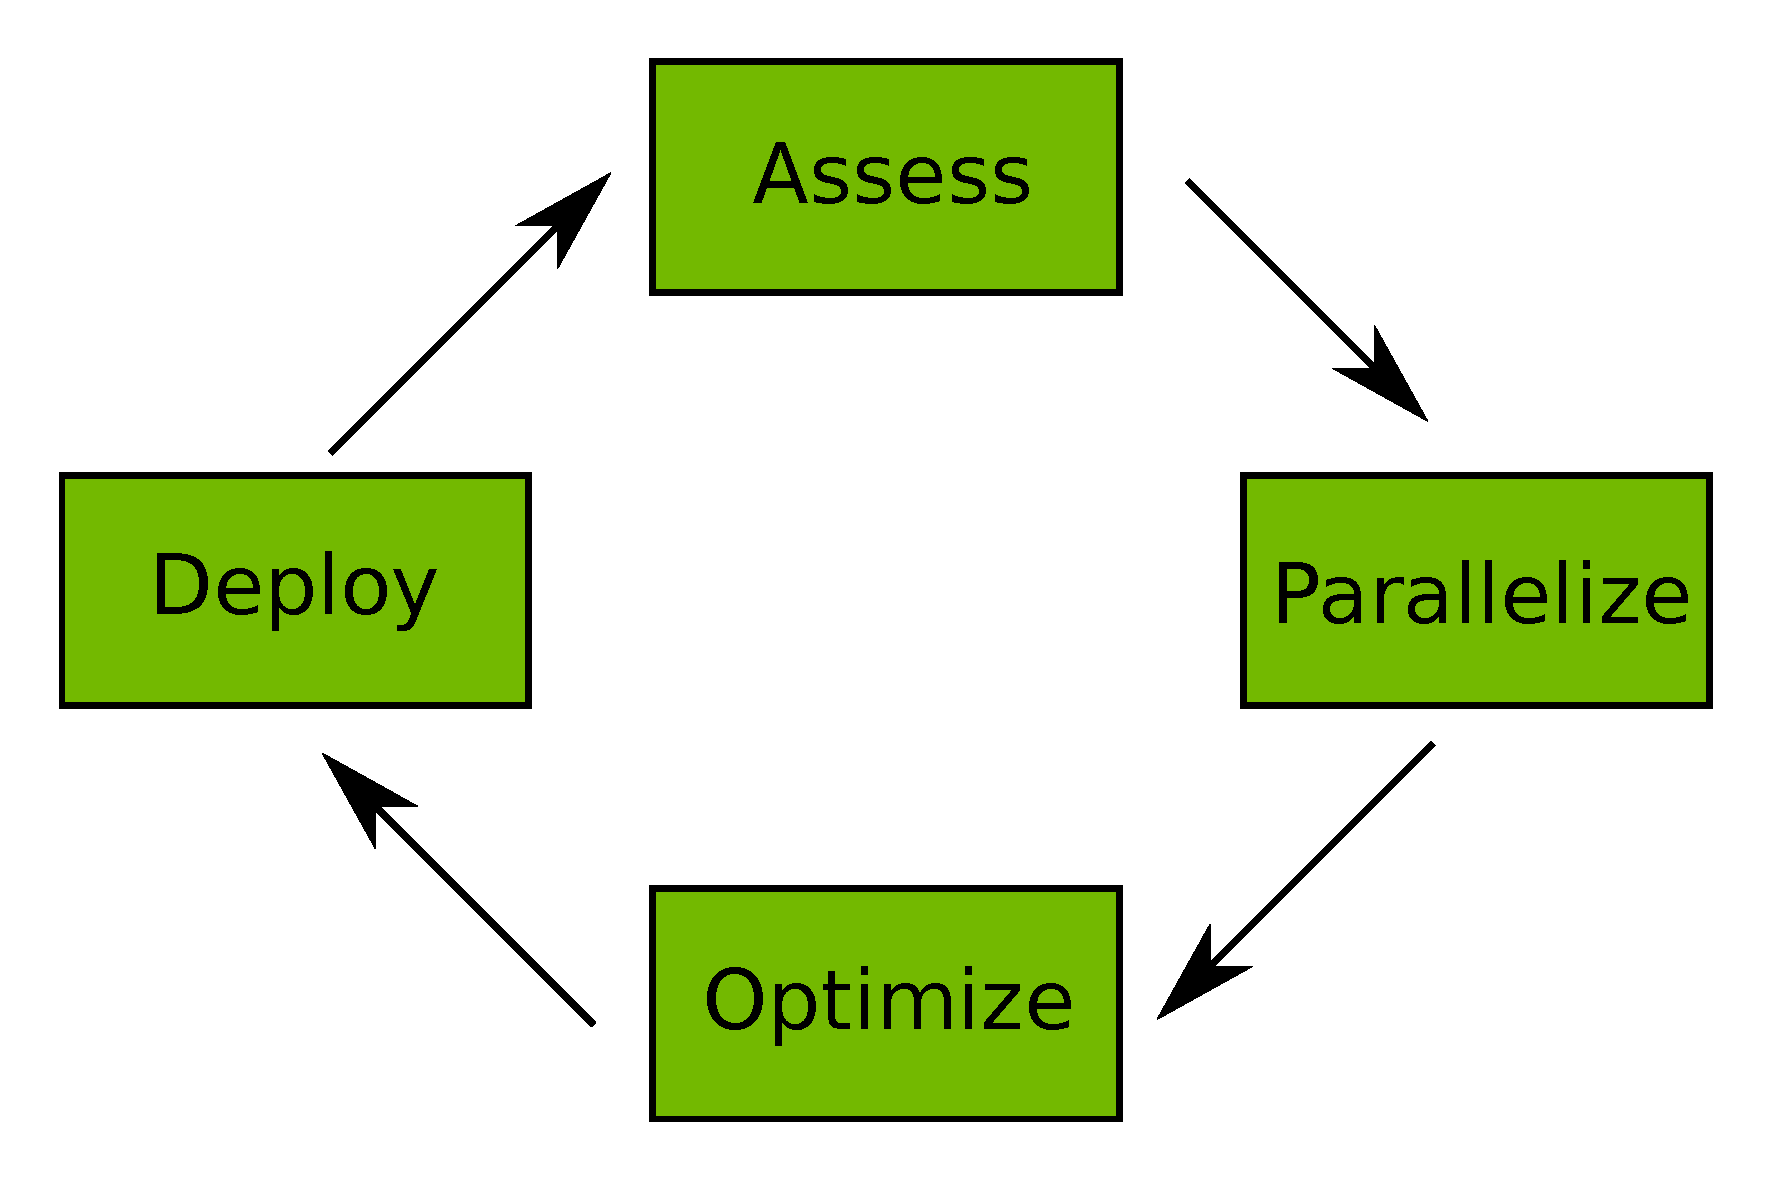
\includegraphics[scale=0.3]{figures/APOD.pdf}
	\end{figure}
\end{frame}

\begin{frame}{New devices}
	\begin{figure}
		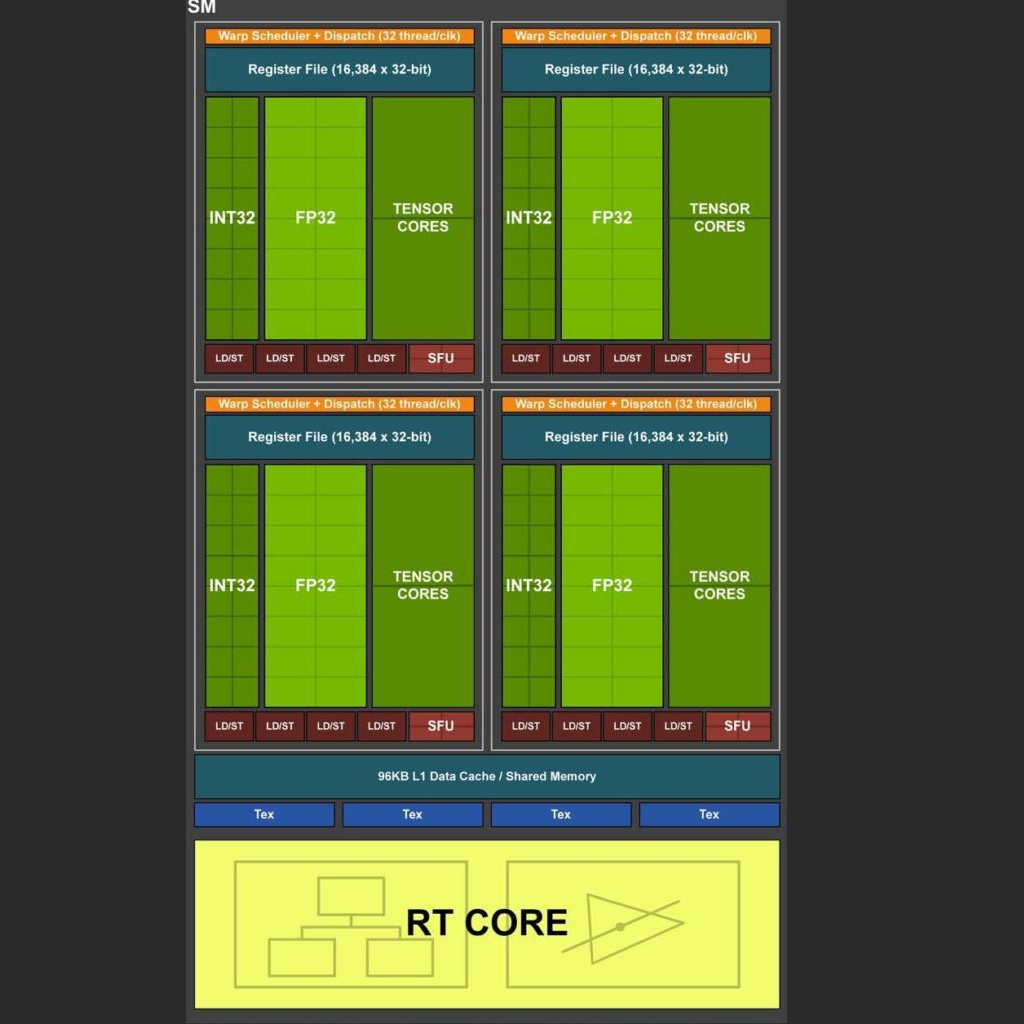
\includegraphics[scale=0.3]{figures/TU102_SM.png}
	\end{figure}
\end{frame}

\begin{frame}{RT cores}
	\begin{figure}
		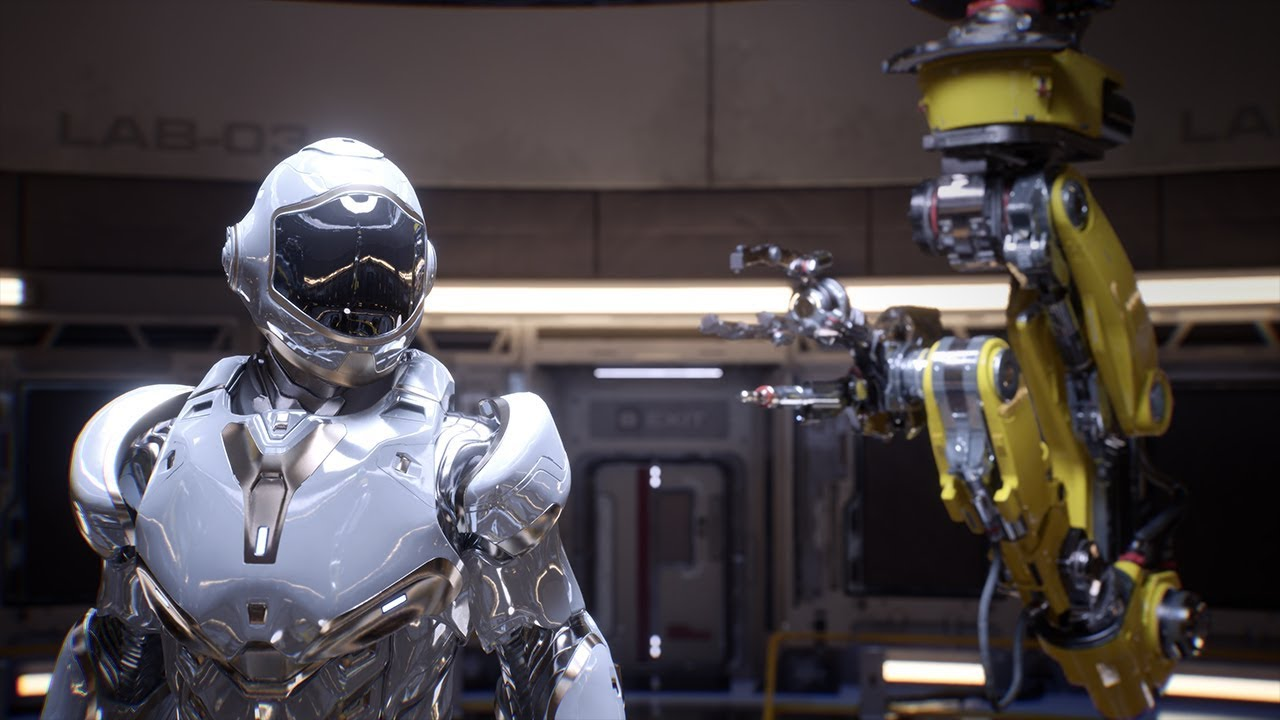
\includegraphics[scale=0.25]{figures/sol.jpg}
	\end{figure}
\end{frame}

\begin{frame}{tensor cores}
	\begin{figure}
		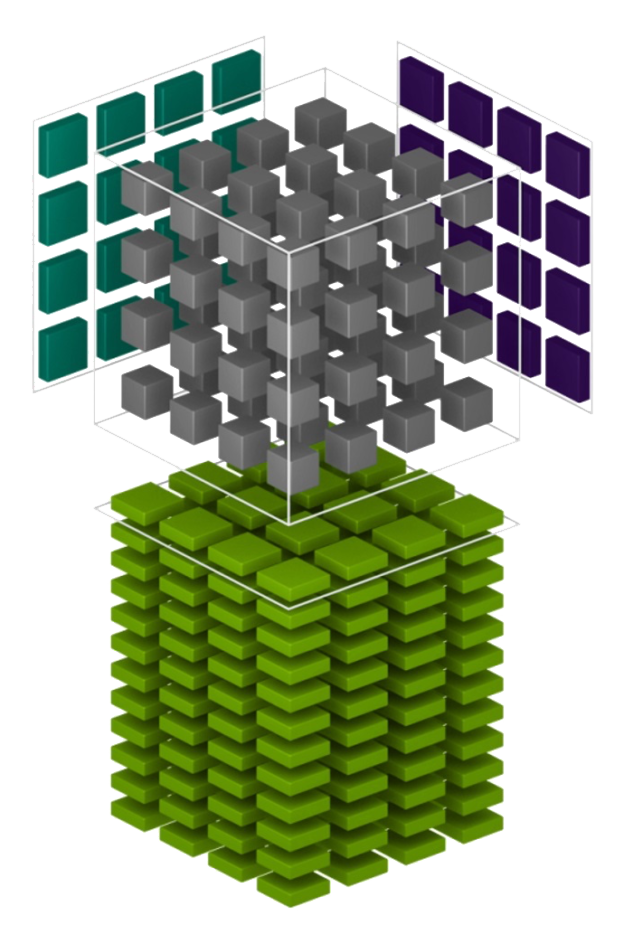
\includegraphics[scale=0.25]{figures/tensor.png}
	\end{figure}
\end{frame}

\begin{frame}{Domain Specific}
	\begin{itemize}
		\item Rendering
		\item Deep Learning
		\item Linear Algebra and Math: Solver, Random function, Finite element method, etc...
		\item Signal
		\item Image and video
		\item Data oriented algorithm
	\end{itemize}
\end{frame}

\section{Example}

\defverbatim[colored]\codeExampleOne{
\begin{lstlisting}
float mean = 0.f;
for(int i=0; i<image_line_size; ++i) {
	mean += 
		image[blockIdx * blockDim + threadIdx];
}
mean /= image_line_size;
\end{lstlisting}
}

\begin{frame}{Process an image line by line}
\codeExampleOne
How image must be layout to minimize cache miss?
\end{frame}


\defverbatim[colored]\codeExampleTwo{
\begin{lstlisting}
float values[512];
for(int i=0; i<512; ++i) {
	values[i] += 
		input[blockIdx * blockDim + threadIdx];
}
\end{lstlisting}
}

\begin{frame}{How to store a lot of local variables}
\codeExampleTwo

\end{frame}



\section{Q\&A}

\end{document}
